% vim: set textwidth=78 autoindent:

% when the revision of a section has been finalized,
% comment out the following line:
%\updatedisclaimer

\section{Raster Data}\label{sec:rasterdata}
\begin{tabular}{p{3.5cm}p{6cm}p{6cm}}
\multirow{2}{*}{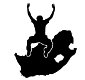
\includegraphics[width=2.5cm]{logo}} & Objectives: &
Understanding what raster data is and how it can be used in a GIS. \\
& & \\
& Keywords: & 
Raster, Pixels, Remote Sensing, Satellite, Image, Georeference  \\
\hline
\end{tabular}

\subsection{Overview}

In the previous topics we have taken a closer look at vector data. While
vector features use geometry (points, polylines and polygons) to represent
the real world, raster data takes a different approach. Rasters are made up
of a matrix of pixels (also called cells), each containing a value that
represents the conditions  for the area covered by that cell (see
Figure \ref{fig:rastergrid}). In this topic we are going to take a closer
look at raster data, when it is useful and when it makes more sense to use
vector data.

\begin{figure}[ht]
   \begin{center}
   \caption{A raster dataset is composed of rows (running across) and columns
(running down) of pixels (also know as cells). Each pixel represents a
geographical region, and the value in that pixel represents some
characteristic of that region.}
\label{fig:rastergrid}\smallskip
   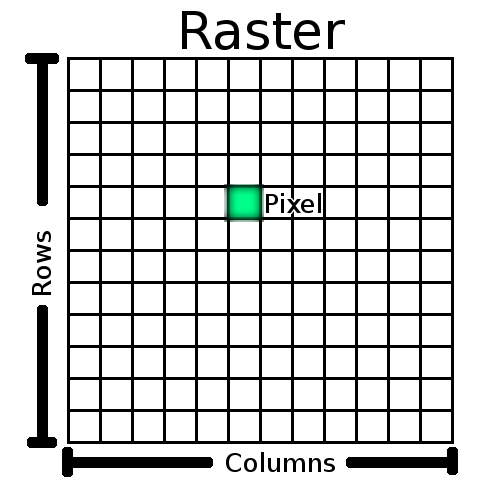
\includegraphics[clip=true, width=0.5\textwidth]{raster_basics}
\end{center}
\end{figure}

\subsection{Raster data in detail}

Raster data is used in a GIS application when we want to display information
that is continuous across an area and cannot easily be divided into vector
features. When we introduced you to vector data we showed you the image in
Figure \ref{fig:landfeatures}. Point, polyline and polygon features work well for
representing some features on this landscape, such as trees, roads and
building footprints. Other features on a landscape can be more difficult to
represent using vector features. For example the grasslands shown have many
variations in colour and density of cover. It would be easy enough to make a
single polygon around each grassland area, but a lot of the information about
the grassland would be lost in the process of simplifying the features to a
single polygon. This is because when you give a vector feature attribute
values, they apply to the whole feature, so vectors aren't very good at
representing features that are not homogeneous (entirely the same) all over.
Another approach you could take is to digitise every small variation of grass
colour and cover as a separate polygon. The problem with that approach is
that it will take a huge amount of work in order to create a good vector
dataset. 

\begin{figure}[ht]
   \begin{center}
   \caption{Some features on a landscape are easy to represent as points,
polylines and polygons (e.g. trees, roads, houses). In other cases it can be
difficult. For example how would you represent the grasslands? As polygons?
What about the variations in colour you can see in the grass? When you are
trying to represent large areas with continuously changing values, raster
data can be a better choice.}
\label{fig:landfeatures}\smallskip
   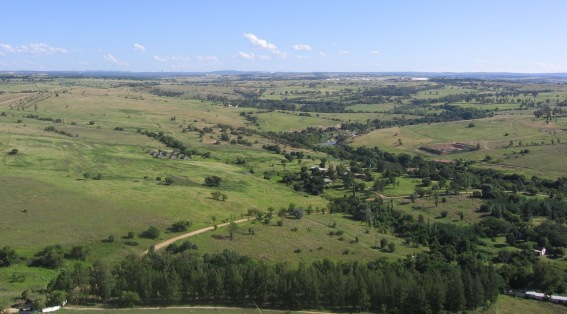
\includegraphics[clip=true, width=\textwidth]{Landscape}
\end{center}
\end{figure}

Using raster data is a solution to these problems. Many people use raster
data as a backdrop to be used behind vector layers in order to provide more
meaning to the vector information. The human eye is very good at interpreting
images and so using an image behind vector layers, results in maps with a lot
more meaning. Raster data is not only good for images that depict the real
world surface (e.g. satellite images and aerial photographs), they are also
good for representing more abstract ideas. For example, rasters can be used
to show rainfall trends over an area, or to depict the fire risk on a
landscape. In these kinds of applications, each cell in the raster represents
a different value. e.g. risk of fire on a scale of one to ten.

An example that shows the difference between an image obtained from a
satellite and one that shows calculated values can be seen in Figure
\ref{fig:imgcomp}.

\begin{figure}[ht]
   \begin{center}
   \caption{True colour raster images (left) are useful as they provide a lot
of detail that is hard to capture as vector features but easy to see when
looking at the raster image. Raster data can also be non-photographic data
such as the raster layer shown on the right which shows the calculated
average minimum temperature in the Western Cape for the month of March.}
\label{fig:imgcomp}\smallskip
   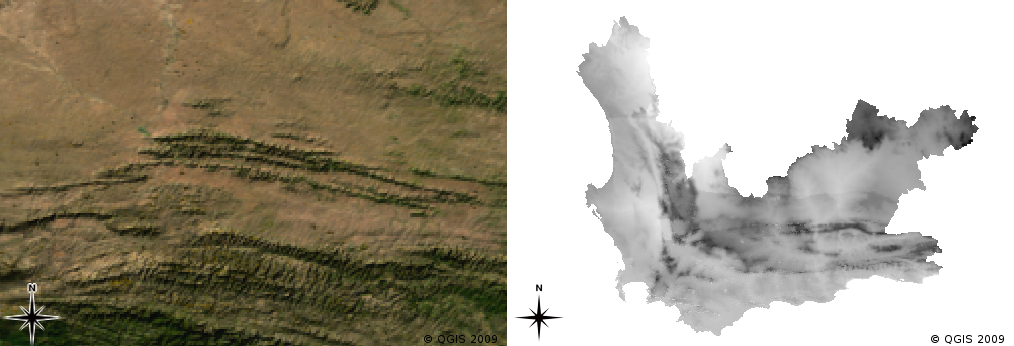
\includegraphics[clip=true, width=\textwidth]{image_vs_computed}
\end{center}
\end{figure}

\subsection{Georeferencing}

Georeferencing is the process of defining exactly where on the earth's
surface an image or raster dataset was created. This positional information
is stored with the digital version of the aerial photo. When the GIS
application opens the photo, it uses the positional information to ensure
that the photo appears in the correct place on the map. Normally this
positional information consists of a coordinate for the top left pixel in the
image, the size of each pixel in the X direction, the size of each pixel in
the Y direction, and the amount (if any) by which the image is rotated. With
these few pieces of information, the GIS application can ensure that raster
data are displayed in the correct place. The georeferencing information for a
raster is often provided in a small text file accompanying the raster.

\subsection{Sources of raster data}

Raster data can be obtained in a number of ways. Two of the most common ways
are aerial photography and satellite imagery. In aerial photography, an
aeroplane flies over an area with a camera mounted underneath it. The
photographs are then imported into a computer and georeferenced. Satellite
imagery is created when satellites orbiting the earth point special digital
cameras towards the earth and then take an image of the area on earth they
are passing over. Once the image has been taken it is sent back to earth
using radio signals to special receiving stations such as the one shown in
Figure \ref{fig:csir}. The process of capturing raster data from an aeroplane
or satellite is called remote sensing.

\begin{figure}[ht]
   \begin{center}
   \caption{The CSIR Satellite Applications Center at Hartebeeshoek near
Johannesburg. Special antennae track satellites as they pass overhead and
download images using radio waves.}
\label{fig:csir}\smallskip
   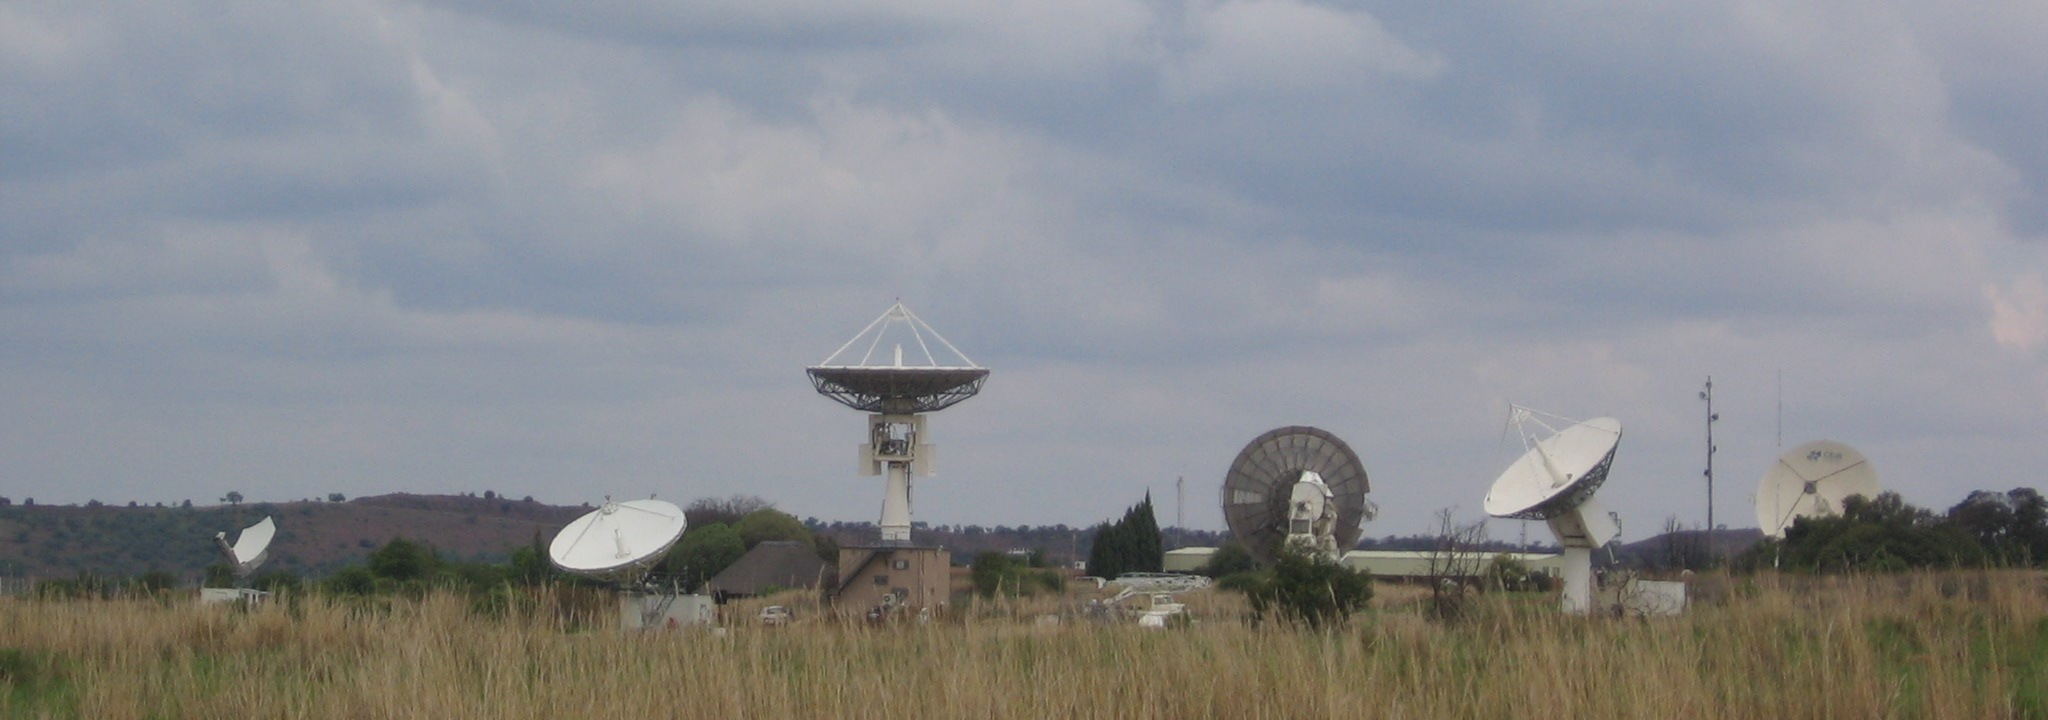
\includegraphics[clip=true, width=\textwidth]{hartebeeshoek}
\end{center}
\end{figure}

In other cases, raster data can be computed. For example an insurance company
may take police crime incident reports and create a country wide raster map
showing how high the incidence of crime is likely to be in each area.
Meteorologists (people who study weather patterns) might generate a  province
level raster showing average temperature, rainfall and wind direction using
data collected from weather stations (see Figure \ref{fig:csir}). In these
cases, they will often use raster analysis techniques such as interpolation
(which we describe in Topic \ref{sec:interpolation}).

Sometimes raster data are created from vector data because the data owners
want to share the data in an easy to use format. For example, a company with
road, rail, cadastral and other vector datasets may choose to generate a
raster version of these datasets so that employees can view these datasets in
a web browser. This is normally only useful if the attributes, that users
need to be aware of, can be represented on the map with labels or symbology.
If the user needs to look at the attribute table for the data, providing it
in raster format could be a bad choice because raster layers do not usually
have any attribute data associated with them.

\subsection{Spatial Resolution}

Every raster layer in a GIS has pixels (cells) of a fixed size that determine
its  spatial resolution. This becomes apparent when you look at an image at a
small scale (see Illustration 5 below) and then zoom in to a large scale (see
Illustration 6 below).

%% Minipage to put both figures on one page
\begin{figure}[htpb]
   \begin{minipage}[h]{\textwidth}
   \begin{center}
   \caption{This satellite image looks good when using a small scale...}
   \label{fig:smallscale}\smallskip
   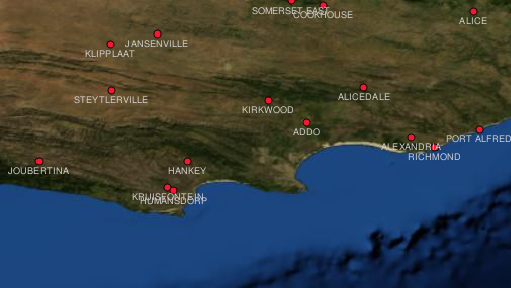
\includegraphics[clip=true, width=0.6\textwidth]{raster_zoomed_out}
   \end{center}
   \end{minipage} \\
   \vspace{1cm}
   \begin{minipage}[h]{\textwidth}
   \begin{center}
   \caption{...but when viewed at a large scale you can see the individual
pixels that the image is composed of.}
   \label{fig:largescale}\smallskip
   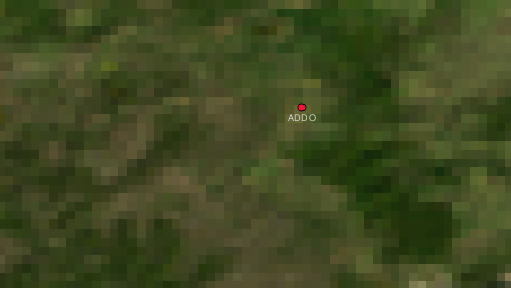
\includegraphics[clip=true, width=0.6\textwidth]{raster_zoomed_in}
   \end{center}
   \end{minipage}
\end{figure}

Several factors determine the spatial resolution of an image. For remote
sensing data, spatial resolution is usually determined by the capabilities of
the sensor used to take an image. For example SPOT5 satellites can take
images where each pixel is 10m x 10m. Other satellites, for example MODIS
take images only at 500m x 500m per pixel. In aerial photography, pixel sizes
of 50cm x 50cm are not uncommon. Images with a pixel size covering a small
area are called \textbf{'high resolution'} images because it is possible to
make out a high degree of detail in the image. Images with a pixel size
covering a large area are called \textbf{'low resolution'} images because the
amount of detail the images show is low.

In raster data that is computed by spatial analysis (such as the rainfall map
we mentioned earlier), the spatial density of information used to create the
raster will usually determine the spatial resolution. For example if you want
to create a high resolution average rainfall map, you would ideally need many
weather stations in close proximity to each other.

One of the main things to be aware of with rasters captured at a high spatial
resolution is storage requirements. Think of a raster that is 3x3 pixels,
each of which contains a number representing average rainfall. To store all
the information contained in the raster, you will need to store 9 numbers in
the computer's memory. Now imagine you want to have a raster layer for the
whole of South Africa with pixels of 1km x 1km. South Africa is around
1,219,090 km2. Which means your computer would need to store over a million
numbers on its hard disk in order to hold all of the information. Making the
pixel size smaller would greatly increase the amount of storage needed.

Sometimes using a low spatial resolution is useful when you want to work with
a large area and are not interested in looking at any one area in a lot of
detail. The cloud maps you see on the weather report, are an example of this
- it's useful to see the clouds across the whole country. Zooming in to one
particular cloud in high resolution will not tell you very much about the
upcoming weather!

On the other hand, using low resolution raster data can be problematic if you
are interested in a small region because you probably won't be able to make
out any individual features from the image.

\subsection{Spectral resolution}

If you take a colour photograph with a digital camera or camera on a
cellphone, the camera uses electronic sensors to detect red, green and blue
light. When the picture is displayed on a screen or printed out, the red,
green and blue (RGB) information is combined to show you an image that your
eyes can interpret. While the information is still in digital format though,
this RGB information is stored in separate colour \textbf{bands}. 

Whilst our eyes can only see RGB wavelengths, the electronic sensors in
cameras are able to detect wavelengths that our eyes cannot. Of course in a
hand held camera it probably doesn't make sense to record information from
the \textbf{non-visible} parts of the spectrum since most people just want to
look at
pictures of their dog or what have you. Raster images that include data for
non-visible parts of the light spectrum are often referred to as
multi-spectral images. In GIS recording the non-visible parts of the spectrum
can be very useful. For example, measuring infra-red light can be useful in
identifying water bodies. 

Because having images containing multiple bands of light is so useful in GIS,
raster data are often provided as multi-band images. Each band in the image
is like a separate layer. The GIS will combine three of the bands and show
them as red, green and blue so that the human eye can see them. The number of
bands in a raster image is referred to as its \textbf{spectral resolution}.

If an image consists of only one band, it is often called a grayscale image.
With grayscale images, you can apply false colouring to make the differences
in values in the pixels more obvious. Images with false colouring applied are
often referred to as \textbf{pseudocolour images}.

\subsection{Raster to vector conversion}

In our discussion of vector data, we explained that often raster data are
used as a backdrop layer, which is then used as a base from which vector
features can be digitised.

Another approach is to use advanced computer programs to automatically
extract vector features from images. Some features such as roads show in an
image as a sudden change of colour from neighbouring pixels. The computer
program looks for such colour changes and creates vector features as a
result. This kind of functionality is normally only available in very
specialised (and often expensive) GIS software.

\subsection{Vector to raster conversion}

Sometimes it is useful to convert vector data into raster data. One side
effect of this is that attribute data (that is attributes associated with the
original vector data) will be lost when the conversion takes place. Having
vectors converted to raster format can be useful though when you want to give
GIS data to non GIS users. With the simpler raster formats, the person you
give the raster image to can simply view it as an image on their computer
without needing any special GIS software.

\subsection{Raster analysis}

There are a great many analytical tools that can be run on raster data which
cannot be used with vector data. For example, rasters can be used to model
water flow over the land surface. This information can be used to calculate
where watersheds and stream networks exist, based on the terrain.

Raster data are also often used in agriculture and forestry to manage crop
production. For example with a satellite image of a farmer's lands, you can
identify areas where the plants are growing poorly and then use that
information to apply more fertilizer on the affected areas only. Foresters
use raster data to estimate how much timber can be harvested from an area.

Raster data is also very important for disaster management. Analysis of
Digital Elevation Models (a kind of raster where each pixel contains the
height above sea level) can then be used to identify areas that are likely to
be flooded. This can then be used to target rescue and relief efforts to
areas where it is needed the most.

\subsection{Common problems / things to be aware of}

As we have already mentioned, high resolution raster data can require large
amounts of computer storage.

\subsection{What have we learned?}

Let's wrap up what we covered in this worksheet:

\begin{itemize}
\item Raster data are a grid of regularly sized \textbf{pixels}.
\item Raster data are good for showing \textbf{continually varying
information}.
\item The size of pixels in a raster determines its \textbf{spatial
resolution}.
\item Raster images can contain one or more \textbf{bands}, each covering the
same spatial area, but containing different information.
\item When raster data contains bands from different parts of the electromagnetic
spectrum, they are called \textbf{multi-spectral images}.
\item Three of the bands of a multi-spectral image can be shown in the colours Red,
Green and Blue so that we can see them.
\item Images with a single band are called grayscale images.
\item Single band, grayscale images can be shown in pseudocolour by the GIS.
\item Raster images can consume a large amount of storage space.
\end{itemize}

\subsection{Now you try!}

Here are some ideas for you to try with your learners:

\begin{itemize}
\item Discuss with your learners in which situations you would use raster
data and in which you would use vector data.
\item Get your learners to create a raster map of your school by using  A4
transparency sheets with grid lines drawn on them. Overlay the transparencies
onto a toposheet or aerial photograph of your school. Now let each learner or
group of learners colour in cells that represent a certain type of feature.
e.g. building, playground, sports field, trees, footpaths etc. When they are
all finished, overlay all the sheets together and see if it makes a good
raster map representation of your school. Which types of features worked well
when represented as rasters? How did your choice in cell size affect your
ability to represent different feature types?
\end{itemize}

\subsection{Something to think about}

If you don't have a computer available, you can understand raster data using
pen and paper. Draw a grid of squares onto a sheet of paper to represent your
soccer field. Fill the grid in with numbers representing values for grass
cover on your soccer field. If a patch is bare give the cell a value of 0. If
the patch is mixed bare and covered, give it a value of 1. If an area is
completely covered with grass, give it a value of 2. Now use pencil crayons
to colour the  cells based on their values. Colour cells with value 2 dark
green. Value 1 should get coloured light green, and value 0 coloured in
brown. When you finish, you should have a raster map of your soccer field!


\subsection{Further reading}

\textbf{Book}:
 
Chang, Kang-Tsung (2006): Introduction to Geographic Information Systems. 3rd
Edition.  McGraw Hill. (ISBN 0070658986)
DeMers, Michael N. (2005): Fundamentals of Geographic Information Systems.
3rd Edition. Wiley. (ISBN 9814126195)

\textbf{Website}: \url{http://en.wikipedia.org/wiki/GIS#Raster}


The QGIS User Guide also has more detailed information on working with raster
data in QGIS.

\subsection{What's next?}

In the section that follows we will take a closer look at topology to see how
the relationship between vector features can be used to ensure the best data
quality.


